% =========================================================
% The Lazaros--Eudora Method (LEM) -- Paper I
% lem_paper_final_v4.tex
%
% Reconstructed source, in content parity with the published
% PDF (lem_paper_final_v3.pdf, Zenodo DOI 10.5281/zenodo.19266201).
%
% Changes relative to the published v3 PDF are BIBLIOGRAPHIC ONLY:
%   (a) Sec. 4.2.1: ripser now cites Bauer (2021) + Tralie et al. (2018),
%       previously mis-cited to Gardinazzi et al.
%   (b) Sec. 5.3: "Chia and Pan" -> "Chia et al." (paper has three authors)
%   (c) references.bib: gardinazzi2024persistent author order corrected;
%       chia2025probing added.
% No textual, structural, or theoretical content was altered.
% =========================================================

\documentclass[11pt]{article}

\usepackage[utf8]{inputenc}
\usepackage[T1]{fontenc}
\usepackage{amsmath, amssymb, amsthm}
\usepackage{graphicx}
\usepackage{booktabs}
\usepackage{enumitem}
\usepackage[margin=1in]{geometry}
\usepackage{cite}
\usepackage{hyperref}

\hypersetup{
  colorlinks = true,
  linkcolor  = black,
  citecolor  = black,
  urlcolor   = blue
}

\title{The Lazaros--Eudora Method (LEM):\\
A Topological Framework for User--LLM Interaction Dynamics}

\author{Lazaros Varvatis}
\date{}

\begin{document}
\maketitle

% =========================================================
% ABSTRACT
% =========================================================

\begin{abstract}
We introduce the Lazaros--Eudora Method (LEM), a conceptual and computational
framework for analyzing user--LLM interactions as dynamic trajectories in latent
representation space rather than as isolated prompt--response pairs. The central
hypothesis of LEM is that repeated interaction between a user and a language
model induces structured trajectory regimes that can be described through
user-specific attractors and compact interaction signatures. We argue that purely
geometric similarity is insufficient for characterizing such regimes and motivate
a topological reformulation based on persistent homology. To render the framework
testable without reliance on proprietary frontier-model internals, we present two
toy-model validations in controlled synthetic settings. The first demonstrates
geometric identifiability of user-conditioned trajectories in a controlled latent
dynamical system, achieving perfect nearest-neighbor re-identification in the
reported synthetic setting across $N=500$ users and ten independent random seeds,
compared to a random baseline of $0.002$. The second shows that convergent and
cyclic interaction regimes can be distinguished through persistent $H_1$ structure
after noisy projection into a higher-dimensional latent space, yielding a
signal-to-noise ratio of $161.6$. We position LEM as a testable research program
for studying user--LLM interaction dynamics, while explicitly delimiting its
current scope and empirical constraints.
\end{abstract}

% =========================================================
% 1. INTRODUCTION
% =========================================================

\section{Introduction}

Current large language model evaluation remains dominated by static, turn-local
metrics. These metrics can assess answer quality, benchmark performance, or
stylistic alignment, but they do not directly describe the temporal structure of
repeated user--model interaction. As a result, an important object remains
under-modeled: the trajectory induced by a specific user interacting with a model
across multiple turns.

The Lazaros--Eudora Method (LEM) is a framework designed to study this object. Its
central premise is that user--LLM interaction should be modeled as a dynamical
trajectory in latent space rather than as a collection of isolated prompt
embeddings or output tokens. In this view, repeated interaction may generate
structured regimes---for example convergence, recurrence, or instability---that
are more naturally described in the language of dynamical systems and topology
than in the language of static vector similarity alone.

This paper makes a limited but concrete contribution. It does not claim to
establish a full theory of human cognition or a validated description of real
frontier-model internals. Instead, it contributes:

\begin{enumerate}[leftmargin=1.8em]
  \item a compact conceptual formalization of LEM;
  \item a distinction between geometric and topological notions of interaction
        signatures;
  \item two toy-model validations showing how user-conditioned attractors and
        trajectory classes can be operationalized in controlled synthetic
        settings.
\end{enumerate}

The intended contribution is therefore methodological: to provide a testable
framework for studying user--LLM interaction dynamics and to identify which parts
of the theory are already operational, which remain open, and which are presently
speculative.

% =========================================================
% 2. CONCEPTUAL FRAMEWORK
% =========================================================

\section{Conceptual Framework}

\subsection{Interaction trajectories}

We define an interaction trajectory as a time-ordered sequence of states
\[
  x_1, x_2, \ldots, x_T \in \mathcal{X},
\]
where $\mathcal{X}$ is a latent or constructed representation space associated with
a multi-turn user--LLM interaction. In practice, $\mathcal{X}$ may refer to internal
activations, reduced coordinates, or synthetic latent states in a toy model.

This shift from isolated states to trajectories is the first core move of LEM. The
object of study is not merely the embedding of a prompt or response, but the path
induced by repeated interaction.

\subsection{Cognitive signatures}

A \emph{cognitive signature} is a compact representation derived from an
interaction trajectory that preserves salient structural properties of user--model
dynamics. In the present paper, we distinguish two operational levels:

\begin{enumerate}[leftmargin=1.8em]
  \item \textbf{Geometric signatures}, defined through distances, directional
        similarity, and nearest-neighbor re-identification in a controlled latent
        system;
  \item \textbf{Topological signatures}, defined through persistent homology,
        especially the presence or absence of robust $H_1$ features.
\end{enumerate}

This distinction is essential. Geometric signatures capture identifiability in a
vector-space sense. Topological signatures capture regime structure that may not
be reducible to distance alone.

\subsection{Attractor-like interaction regimes}

LEM uses the term \emph{attractor} in a modeling sense. The claim is not that real
human cognition has been recovered from LLM traces, but that repeated interaction
can be approximated as a dynamical process whose trajectories may approach stable
regimes. In the minimal setting considered here, these include:

\begin{itemize}[leftmargin=1.8em]
  \item \textbf{Convergent regimes}, approximated by a stable fixed point;
  \item \textbf{Cyclic regimes}, approximated by a stable limit cycle;
  \item \textbf{Unstable or noisy regimes}, in which no compact structural summary
        is stable.
\end{itemize}

\subsection{Core hypotheses}

We focus on four hypotheses, of which only the first three are partially
operationalized in the current paper.

\paragraph{H1: Geometric identifiability.}
User-conditioned interaction dynamics can generate trajectories that are
re-identifiable above chance in a controlled latent system.

\paragraph{H2: Regime differentiation.}
Convergent and cyclic interaction regimes generate structurally distinct trajectory
classes.

\paragraph{H3: Topological utility.}
Persistent homology captures structural differences between such regimes, especially
through the presence or absence of persistent $H_1$ features.

\paragraph{H4: Cross-version stability.}
User-specific interaction signatures may remain partially stable across related
model variants or model families. In this paper, H4 is treated as a theoretical
target rather than an empirically established claim.

% =========================================================
% 3. FROM GEOMETRIC SIMILARITY TO TOPOLOGICAL STRUCTURE
% =========================================================

\section{From Geometric Similarity to Topological Structure}

Many current approaches to personalization, user modeling, and dialogue adaptation
rely on static similarity measures, clustering, or compressed user embeddings.
These approaches are useful, but they typically summarize multi-turn interaction as
a point estimate or a low-order statistic.

LEM instead treats interaction as a trajectory and therefore distinguishes between
two levels of structure:

\begin{enumerate}[leftmargin=1.8em]
  \item \textbf{Geometric structure}: whether trajectories lie near each other or
        near user-conditioned attractors;
  \item \textbf{Topological structure}: whether trajectories exhibit recurrence,
        loop-like organization, or topological triviality.
\end{enumerate}

This motivates the use of topological data analysis (TDA), especially persistent
homology. In the current work, the key topological observable is persistent $H_1$
structure, interpreted as evidence of recurrent cyclic organization in trajectory
point clouds.

We explicitly do \emph{not} claim that topological features directly reveal
psychological essence or consciousness. The intended claim is narrower: in a
controlled setting, topology can distinguish classes of interaction dynamics that
are poorly summarized by static geometry alone.

% =========================================================
% 4. TOY-MODEL NUMERICAL VALIDATION
% =========================================================

\section{Toy-Model Numerical Validation}

The present paper does not attempt to validate LEM directly on proprietary
frontier-model internals. Instead, it follows a more modest and methodologically
transparent strategy: we test whether the core conceptual claims of the framework
can be operationalized in controlled synthetic systems. The goal of these toy
experiments is not realism, but falsifiability. If the central vocabulary of
LEM---user-conditioned trajectories, attractor-like behavior, and topological
regime separation---cannot be instantiated even in simple latent dynamical systems,
the framework would lack methodological credibility.

We therefore use two toy experiments with distinct roles. The first tests
\emph{geometric identifiability}: whether user-conditioned latent dynamics generate
re-identifiable trajectories above chance. The second tests \emph{topological class
separation}: whether convergent and cyclic regimes remain distinguishable after
projection into a noisy higher-dimensional latent space.

% ---------------------------------------------------------
\subsection{Toy Experiment 1: Geometric Identifiability}

The first toy experiment is a geometric sanity check for the notion of
user-specific interaction structure. We consider a latent dynamical system of the
form
\begin{equation}
  x_{t+1} = (1 - \alpha - \beta)\, x_t + \alpha\, s_i + \beta\, d_m + \varepsilon_t,
\end{equation}
where $x_t \in \mathbb{R}^d$ denotes the latent state at time $t$, $s_i$ is a
user-specific signature vector, $d_m$ is a domain or model attractor, and
$\varepsilon_t \sim \mathcal{N}(0, \sigma^2 I_d)$ is isotropic Gaussian noise. The
interpretation is deliberately minimal: $s_i$ models a user-conditioned directional
bias in latent space, while $d_m$ models task- or model-level regularization toward
a shared region. This is a controlled synthetic separability regime and does not
simulate a deployed user--model interaction.

\subsubsection{Setup}

We instantiate $N=500$ users and $M=2$ model domains in a $d=512$-dimensional
embedding space. User signature vectors $s_i \sim \mathcal{N}(0, I_d)$ and domain
attractors $d_m \sim \mathcal{N}(0, I_d)$ are sampled independently and
$\ell_2$-normalised. Trajectories are simulated with $\alpha=0.4$, $\beta=0.3$,
$\sigma=0.15$, and $T=200$ time steps. Empirical user signatures are estimated as
\begin{equation}
  \hat{s}^{(m)}_i = \frac{1}{K} \sum_{t=T-K}^{T} x^{(i,m)}_t - \beta\, d_m,
  \qquad K=40.
\end{equation}
In the noise-free expectation, the deterministic fixed point of Eq.~(1) is
\begin{equation}
  x^{*} = \frac{\alpha\, s_i + \beta\, d_m}{\alpha + \beta}.
\end{equation}
All experiments are repeated over ten independent random seeds
$\{42, 123, 999, 2024, 7, 314, 1337, 77, 256, 88\}$.

\subsubsection{Metrics}

We evaluate three observables: (i) mean $\ell_2$ distance between the empirical
trajectory mean and the theoretical fixed point of Eq.~(3); (ii) nearest-neighbor
re-identification accuracy over $N_{\text{test}}=500$ fresh test queries per model;
(iii) same-user versus different-user cosine similarity of empirical signatures
across model domains.

\subsubsection{Results}

Table~\ref{tab:toy1} reports summary statistics across all ten seeds.

\begin{table}[htbp]
  \centering
  \caption{Toy Experiment 1 --- scaled results in the controlled synthetic
           separability regime ($d$=512, $N$=500, $T$=200, 10 seeds).}
  \label{tab:toy1}
  \begin{tabular}{lrrrr}
    \toprule
    \textbf{Metric} & \textbf{Mean} & \textbf{Std} & \textbf{Min} & \textbf{Max} \\
    \midrule
    Random baseline accuracy & 0.0020 & ---    & ---     & ---    \\
    NN re-id accuracy        & 1.0000 & 0.0000 & 1.0000  & 1.0000 \\
    Mean attractor distance  & 0.7893 & 0.0009 & 0.7878  & 0.7907 \\
    Cosine (same user)       & 0.3570 & 0.0020 & 0.3538  & 0.3609 \\
    Cosine (different user)  & 0.0022 & 0.0019 & -0.0011 & 0.0056 \\
    \bottomrule
  \end{tabular}
\end{table}

Nearest-neighbor re-identification accuracy reaches $1.000 \pm 0.000$ across all
seeds---a $500\times$ improvement over the random baseline of $0.002$ in this
synthetic setting. Same-user cosine similarity ($0.357 \pm 0.002$) is far above the
near-zero cross-user similarity ($0.002 \pm 0.002$), confirming geometric
separability.

\begin{figure}[htbp]
  \centering
  
\includegraphics[width=\textwidth]{toy_v1_scaled_results.png}
  \caption{Toy Experiment 1. \textbf{Left:} NN re-identification accuracy across ten
           seeds (orange line = mean, red dashed = random baseline).
           \textbf{Right:} cosine similarity for same-user (green) versus
           different-user (red) signature pairs. All results are within the
           controlled synthetic separability regime described in Section~4.1.}
  \label{fig:toy1}
\end{figure}

\subsubsection{Robustness analysis}

To preempt concerns about noise sensitivity, we vary
$\sigma \in \{0.05, 0.15, 0.30, 0.50, 0.75, 1.00, 1.50, 2.00\}$ with all other
parameters fixed (seed $=42$).

\begin{table}[htbp]
  \centering
  \caption{Robustness to noise level $\sigma$ ($d$=512, $N$=500, seed $=$ 42).}
  \label{tab:toy1b}
  \begin{tabular}{rrrrr}
    \toprule
    $\sigma$ & \textbf{NN Acc.} & \textbf{Attr. Dist.} & \textbf{Cos. (same)}
             & \textbf{Cos. (diff)} \\
    \midrule
    0.05 & \textbf{1.0000} & 0.3319  & 0.8037 & 0.0045 \\
    0.15 & \textbf{1.0000} & 0.7895  & 0.3545 & 0.0019 \\
    0.30 & 0.2300          & 1.5348  & 0.1219 & 0.0006 \\
    0.50 & 0.0200          & 2.5419  & 0.0469 & 0.0002 \\
    0.75 & 0.0050          & 3.8054  & 0.0207 & 0.0001 \\
    1.00 & 0.0033          & 5.0703  & 0.0112 & 0.0000 \\
    1.50 & 0.0033          & 7.6017  & 0.0043 & 0.0000 \\
    2.00 & 0.0017          & 10.1339 & 0.0018 & 0.0000 \\
    \bottomrule
  \end{tabular}
\end{table}

\begin{figure}[htbp]
  \centering
  
\includegraphics[width=\textwidth]{toy_v1b_robustness.png}
  \caption{Robustness of LEM signatures to noise $\sigma$. \textbf{Left:} NN accuracy
           with phase transition at $\sigma \approx 0.25$. \textbf{Centre:} attractor
           distance (linear in $\sigma$). \textbf{Right:} cosine separability
           collapse.}
  \label{fig:toy1b}
\end{figure}

Figure~\ref{fig:toy1b} reveals three regimes: a stable regime ($\sigma \leq 0.15$)
with perfect re-identification; a critical transition at $\sigma \approx 0.20$--$0.30$
where accuracy drops sharply; and a noise-dominated regime ($\sigma \geq 0.50$) where
accuracy collapses to baseline. Attractor distance grows linearly with $\sigma$
(slope $\approx 5.07$), consistent with the theoretical prediction
$\|\hat{x}^{*} - x^{*}\| \propto \sigma/(\alpha+\beta)$. Cross-user cosine similarity
remains at $\approx 0$ throughout, confirming that signature confusion rather than
mere degradation drives the accuracy collapse.

The perfect re-identification at $d=512$ reflects the \emph{blessing of
dimensionality}: in high-dimensional spaces, random unit vectors are nearly
orthogonal, rendering user signatures geometrically separable under moderate noise.
This separability is a property of the high-dimensional synthetic construction and
should not be interpreted as evidence that real deployed users are identifiable by
such means. The sharp phase transition at $\sigma \approx 0.25$ defines a clear
operating regime for the LEM and provides a principled criterion for when geometric
identifiability can be expected to hold in controlled settings.

% ---------------------------------------------------------
\subsection{Toy Experiment 2: Topological Class Separation}

The second toy experiment is the central numerical validation for the topological
reformulation of LEM. Here, the aim is not to separate users geometrically, but to
distinguish qualitatively different \emph{dynamical regimes} through topological
invariants.

\subsubsection{Setup}

We construct two synthetic trajectory classes:

\begin{enumerate}[leftmargin=1.8em]
  \item a \textbf{convergent regime}, modeled as a stable sink in two dimensions:
        \begin{equation}
          \dot{x} = -\lambda x, \quad \dot{y} = -\lambda y, \quad \lambda = 0.5,
        \end{equation}
        initialised at $(x_0, y_0) = (2.0,\ 1.5)$;
  \item a \textbf{cyclic regime}, modeled as a stable limit cycle via the Van der Pol
        oscillator:
        \begin{equation}
          \dot{x} = y, \quad \dot{y} = \mu(1 - x^2)y - x, \quad \mu = 1.5,
        \end{equation}
        initialised at $(x_0, y_0) = (0.1,\ 0.1)$.
\end{enumerate}

Both systems are integrated over $T$=40 time units with $\Delta t$=0.1 (401 steps),
then embedded into $\mathbb{R}^{16}$ via a random linear projection
$A \in \mathbb{R}^{2 \times 16}$ with additive Gaussian noise ($\sigma$=0.05).
Persistent homology in degree $H_1$ is computed via the Vietoris--Rips filtration
using \texttt{ripser} \cite{bauer2021ripser,tralie2018ripserpy}.

\subsubsection{Metric}

For each trajectory we compute the degree-1 persistence diagram $\mathrm{PD}(H_1)$.
The key quantity is the \emph{maximum persistence}
\[
  p_{\max} = \max_{(b,d)\, \in\, \mathrm{PD}(H_1)} (d - b),
\]
where $b$ and $d$ denote the birth and death of a homological feature. A large
$p_{\max}$ indicates a robust loop; values near zero indicate no persistent cyclic
structure. We define the signal-to-noise ratio as
\[
  \mathrm{SNR} = \frac{p^{\text{cyclic}}_{\max}}{p^{\text{convergent}}_{\max} + \epsilon},
  \qquad \epsilon = 10^{-9}.
\]

\subsubsection{Results}

\begin{table}[htbp]
  \centering
  \caption{Toy Experiment 2 --- topological class separation ($d$=16, $T$=40,
           seed $=$ 1337).}
  \label{tab:toy2}
  \begin{tabular}{lrr}
    \toprule
    \textbf{Metric} & \textbf{Convergent} & \textbf{Cyclic} \\
    \midrule
    Max $H_1$ persistence     & 0.0326 & 5.2649 \\
    Mean $H_1$ persistence    & 0.0092 & 0.1972 \\
    SNR (cyclic / convergent) & \multicolumn{2}{c}{161.6} \\
    \bottomrule
  \end{tabular}
\end{table}

The cyclic regime produces a maximum $H_1$ persistence of $5.265$, compared to
$0.033$ for the convergent regime---a ratio of $161.6\times$. A simple threshold
classifier at $p_{\max} > 0.1$ separates the two regimes with zero error, requiring
no learned parameters.

These results demonstrate that persistent homology reliably distinguishes convergent
from cyclic LEM dynamics even after noisy high-dimensional embedding, without access
to the original system parameters.

\begin{figure}[htbp]
  \centering
  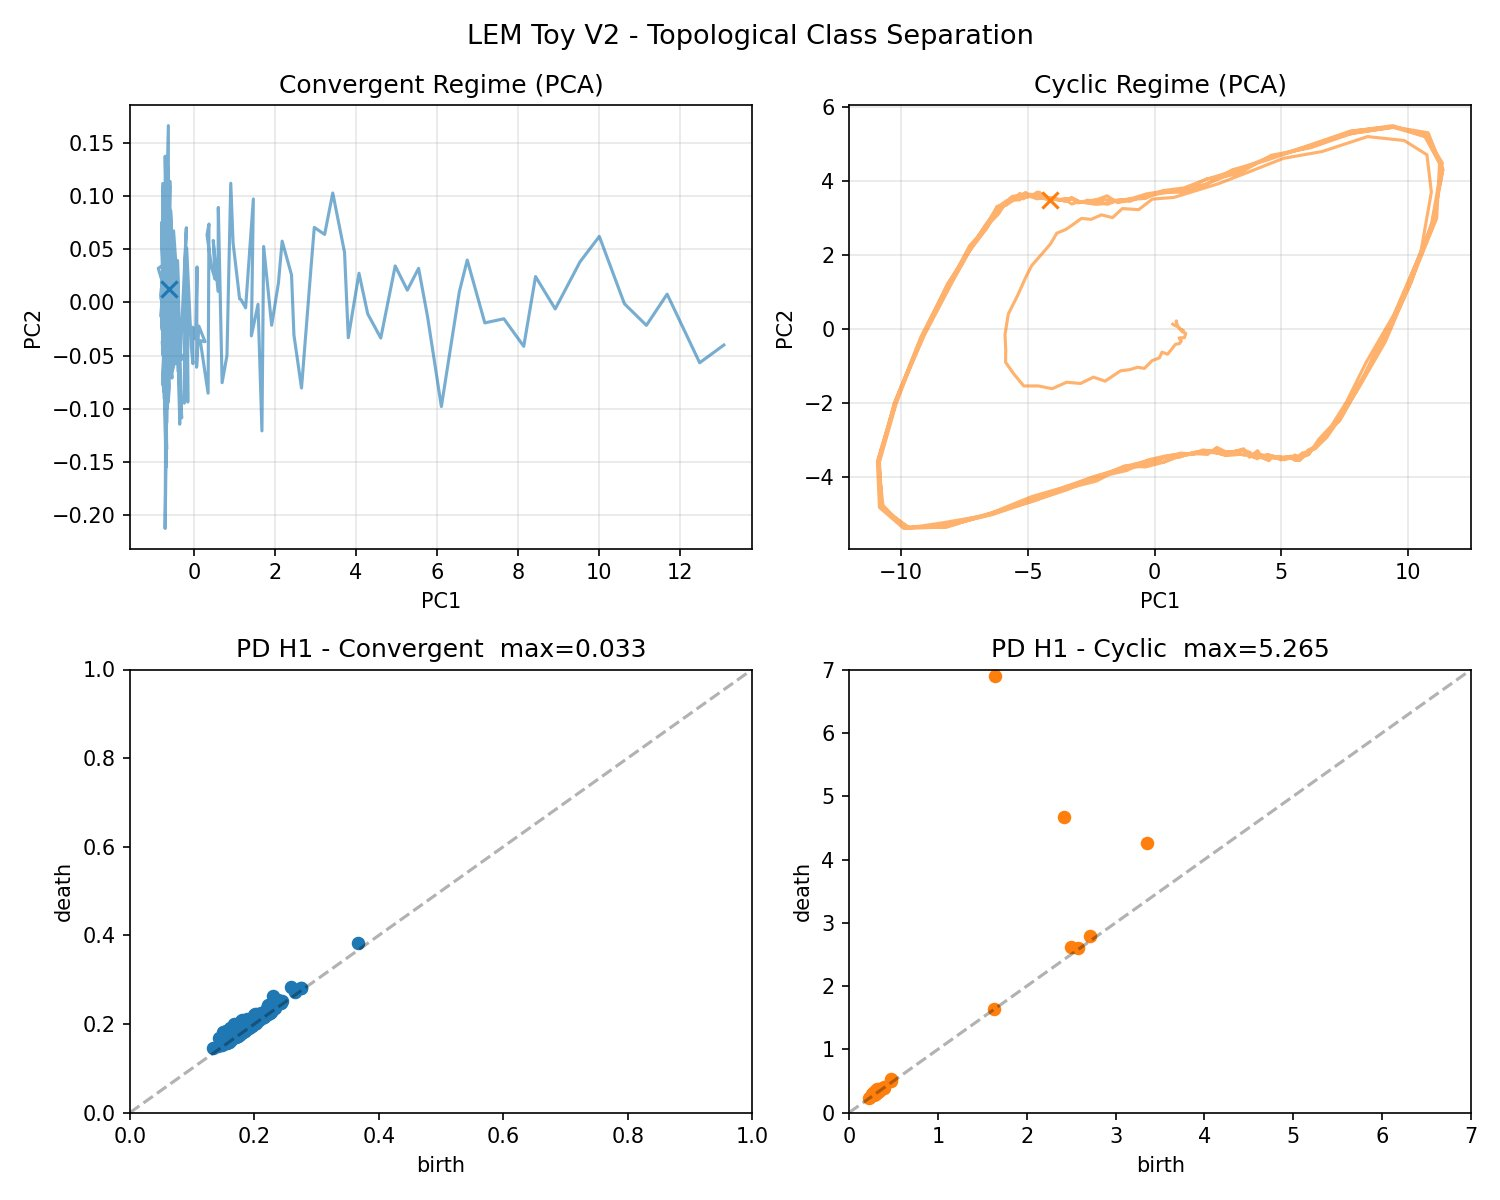
\includegraphics[width=\textwidth]{toy_v2_moneyplot.png}
  \caption{Toy Experiment 2: topological class separation. \textbf{Top:} PCA
           projections of the convergent (left, blue) and cyclic (right, orange)
           trajectories embedded in $\mathbb{R}^{16}$. \textbf{Bottom:} degree-1
           persistence diagrams. The convergent diagram shows only diagonal noise
           ($p_{\max}$=0.033); the cyclic diagram contains a prominent off-diagonal
           generator ($p_{\max}$=5.265) corresponding to the limit-cycle topology.
           SNR $=$ 161.6.}
  \label{fig:toy2}
\end{figure}

% ---------------------------------------------------------
\subsection{What the toy experiments do and do not establish}

Taken together, the two toy experiments support a restricted interpretation of LEM.

\paragraph{Supported in the present paper.}
\begin{itemize}[leftmargin=1.8em]
  \item User-conditioned latent trajectories can be geometrically distinguishable
        above chance in a controlled synthetic separability regime.
  \item Convergent and cyclic trajectory classes can be topologically separated
        through persistent homology (SNR $=$ 161.6).
  \item The vocabulary of attractors, signatures, and topological regime structure
        is operationalizable and falsifiable.
\end{itemize}

\paragraph{Not established in the present paper.}
\begin{itemize}[leftmargin=1.8em]
  \item That real frontier-model activation traces exhibit the same trajectory
        classes.
  \item That interaction signatures correspond to psychological or neuroscientific
        identity.
  \item That high-dimensional synthetic separability implies real-world user
        identifiability.
  \item That cross-version stability has already been demonstrated empirically.
  \item That LEM currently enables deployment-grade personalization, safety, or
        forensic attribution.
\end{itemize}

% =========================================================
% 5. RELATED WORK
% =========================================================

\section{Related Work}

LEM is related to several existing lines of research, but does not coincide exactly
with any single one of them. Its closest neighbors lie in user modeling, latent
behavioral representations, mechanistic interpretability, and topological analysis
of neural representations.

\subsection{User modeling and latent behavioral structure}

A first neighboring tradition concerns latent user representations and
personalization. In these approaches, user-specific state is typically modeled
through compressed embeddings, memory summaries, or preference vectors. LEM is
compatible with this general objective, but differs in one central respect: it
treats repeated user--model interaction not primarily as a static user
representation problem, but as a trajectory-level object. Related work on latent
state persistence in LLMs has raised important questions about whether models
maintain stable internal representations across turns at all
\cite{huang2025latentstate}. LEM does not presuppose that real LLMs do so; rather,
it asks whether the structure of user-conditioned trajectories is detectable if
such persistence were present.

A closer point of contact is recent work on persona vectors. Chen et al. identify
directions in activation space that correspond to behavioral or character
traits---such as sycophancy, hallucination propensity, or harmfulness---and
demonstrate that these directions are causally effective: injecting or suppressing
them during inference predictably alters model behavior \cite{chen2025persona}. This
provides direct empirical evidence that the latent spaces through which LEM posits
user-conditioned trajectories contain structured, behaviorally meaningful geometry.
LEM builds on this foundation but shifts the focus from static trait directions to
the temporal dynamics of repeated interaction trajectories and the possibility of
deriving geometric and topological signatures from them.

\subsection{Mechanistic interpretability and feature geometry}

LEM is also related to mechanistic interpretability work that studies the internal
organization of model representations. In particular, dictionary-learning and
sparse-autoencoder work argues that model activations can be decomposed into more
interpretable features than individual neurons alone
\cite{bricken2023monosemanticity,templeton2024scaling}. These results matter for LEM
because they provide evidence that model representations are structured enough to
support nontrivial latent analyses. A related direction is the literature on
attribution graphs and circuit tracing, which models internal feature interactions
as structured computational pathways \cite{ameisen2025circuittracing}. LEM differs
in being trajectory-centric rather than feature- or circuit-centric.

\subsection{Topological analysis of representation structure}

A third neighboring tradition concerns topological data analysis in machine learning
and language models. The foundational framework for applying persistent homology to
data analysis was established by Carlsson \cite{carlsson2009topology}. More recently,
Gardinazzi et al. apply persistent homology directly to LLM activation spaces across
layers, demonstrating that topological features capture structural properties of
learned representations that linear probes miss \cite{gardinazzi2024persistent}. Tan
et al. extend this direction to reasoning traces \cite{tan2025shape}. In a
complementary line of work, Chia et al. probe latent subspaces of LLMs to identify
adversarial states and demonstrate that structured regions in activation space can be
isolated and manipulated \cite{chia2025probing}. This supports the broader premise
that LLM latent spaces contain exploitable geometric and topological structure. LEM
draws directly from this methodological tradition, especially in its use of persistent
$H_1$ structure to distinguish topologically trivial from recurrent interaction
regimes.

The narrower novelty claim of LEM is therefore not that topology can be applied to
neural representations in general, but that user--LLM interaction can be modeled as a
dynamical trajectory whose regime class may be summarized through geometric and
topological signatures.

\subsection{Dynamical systems and attractor perspectives}

A fourth neighboring tradition treats language models through the lens of dynamical
systems. Ramsauer et al. show that Transformer attention corresponds to the update
rule of modern Hopfield networks, whose energy landscape admits multiple attractor
types \cite{ramsauer2021hopfield}. Bai et al. demonstrate that hidden layers of deep
sequence models can converge to fixed points, formalizing the notion of equilibrium
computation in neural networks \cite{bai2019deq}. Most directly relevant to LEM, Wang
et al. provide empirical evidence that iterative text generation in LLMs converges to
attractor cycles, including two-period limit cycles under successive paraphrasing
\cite{wang2025attractorcycles}. This establishes that attractor dynamics in language
models are not merely a theoretical construct but an empirically observable
phenomenon.

LEM differs from this line of work in three respects. First, it studies
user-conditioned trajectories rather than generic model dynamics. Second, it operates
in latent representation space rather than in text space. Third, it employs
topological analysis to distinguish regime types, whereas existing dynamical-systems
work on LLMs has not used persistent homology for this purpose.

\subsection{Positioning of the present contribution}

The present paper should not be read as claiming to be the first connection between
topology and language models, nor the first work on latent behavioral directions, nor
the first dynamical-systems perspective on LLMs. Each of these components has
established precedent. The narrower contribution of LEM is the synthesis: it
introduces a single trajectory-based framework in which:

\begin{enumerate}[leftmargin=1.8em]
  \item user-conditioned interaction is modeled dynamically (building on
        \cite{wang2025attractorcycles,ramsauer2021hopfield,bai2019deq});
  \item attractor-like behavior becomes a first-class object of analysis, supported
        by evidence that latent spaces encode structured behavioral geometry
        \cite{chen2025persona,bricken2023monosemanticity};
  \item geometric identifiability and topological regime structure are treated
        jointly, using tools from persistent homology
        \cite{carlsson2009topology,gardinazzi2024persistent}.
\end{enumerate}

No existing work in the surveyed literature combines all three elements. LEM is
therefore best understood as a synthesis with a specific new emphasis: the study of
user--LLM interaction through the combined lenses of trajectory dynamics, attractor
structure, and topological signatures.

% =========================================================
% 6. DISCUSSION AND LIMITATIONS
% =========================================================

\section{Discussion and Limitations}

The main contribution of the present formulation is methodological. LEM is strongest
when interpreted not as a completed explanatory theory, but as a compact research
program that introduces a trajectory-based object of analysis and proposes geometric
and topological tools for studying it.

The toy models support two limited claims:

\begin{enumerate}[leftmargin=1.8em]
  \item user-conditioned trajectories can be geometrically identifiable above chance
        in a controlled synthetic separability regime;
  \item convergent and cyclic trajectory classes can be topologically separated
        through persistent homology.
\end{enumerate}

These findings do not establish that real frontier-model interaction traces behave in
the same way. They instead show that the theoretical vocabulary of LEM is
operationalizable and falsifiable in controlled synthetic settings.

It bears emphasis that the perfect re-identification observed in Toy Experiment 1 is
a consequence of the high-dimensional synthetic construction, not evidence for
real-world user fingerprinting. In $d=512$ dimensions, independently sampled random
unit vectors are near-orthogonal by concentration-of-measure arguments, making
separation trivially achievable in the absence of real-world confounds such as
overlapping behavioral styles, model-induced compression, or adversarial noise. The
value of Toy Experiment 1 lies not in the magnitude of the accuracy, but in confirming
that the attractor-based update rule produces stable, structured trajectories in the
controlled regime.

This work has several further limitations. First, all numerical validation is based on
synthetic toy dynamics rather than internal activation traces from real language
models. Second, the notion of an interaction signature is operational and
representational, not psychological or neuroscientific. Third, the current paper does
not establish cross-version or cross-model stability. Fourth, no claim is made here
that topological signatures are already useful for deployed personalization, safety,
or forensic attribution.

The paper deliberately avoids stronger claims about cognition, consciousness, or human
identity. Its scope is restricted to a formal and computational framework for
analyzing interaction dynamics.

% =========================================================
% 7. FUTURE WORK
% =========================================================

\section{Future Work}

There are four immediate next steps:

\begin{enumerate}[leftmargin=1.8em]
  \item extend the toy-model logic to real multi-turn activation traces from
        open-weight language models;
  \item compare geometric and topological signatures more systematically, including
        bottleneck and Wasserstein diagram distances;
  \item operationalize cross-version stability through diagram-based distances or
        related invariants;
  \item connect LEM more explicitly to current interpretability workflows, including
        feature-based and persona-based latent analyses.
\end{enumerate}

More ambitious directions, including cross-model user continuity, privacy
implications, and robust trajectory-level defenses, should be treated as future
hypotheses rather than present conclusions.

The framework documentation and code are available at
\url{https://github.com/LAKITALKS/LEM}. A citable record is archived at Zenodo
(DOI: \href{https://doi.org/10.5281/zenodo.19266201}{10.5281/zenodo.19266201}).

% =========================================================
% 8. CONCLUSION
% =========================================================

\section{Conclusion}

LEM provides a compact and testable framework for analyzing user--LLM interaction
dynamics as trajectories rather than isolated states. Its central contribution is to
combine attractor-based intuition with a topological reformulation that makes
convergent and cyclic regimes measurable in principle. The current paper presents a
first version of this program: conceptual formalization plus toy-model numerical
validation. Whether these ideas scale to real language-model internals remains an
open empirical question. However, even at the present stage, LEM provides a clearer
basis for asking that question in a controlled and scientifically tractable way.

% =========================================================
% REFERENCES
% =========================================================

\bibliographystyle{plain}
\bibliography{references}

\end{document}
